\section{Specific Requirements}
\subsection{External Interface Requirements}
\subsubsection{User Interfaces}
The user interface of eMall is a mobile application, with an easy to use design.
It should be available on every major mobile operating system.
\subsubsection{Hardware Interfaces}
The system is fully operated on the Internet, so it doesn't feature any hardware interface, apart from the mobile device needed to access the service.
%\subsubsection{Software Interfaces}
\subsubsection{Communication Interfaces}
The main communication interfaces of the platform are the users and CPMSs.
The system interacts with users to receive booking requests or to send information, and to CPMSs to receive information about charging stations or to remotely interact with the charging socket.
A different interface is when the system sends push notifications to a user or retrieves the users' location, charging status and schedule.
%%% ==> CPMS
%%%
\subsection{Functional Requirements}
\subsubsection{Use case diagrams}
\begin{enumerate}
    \item \textbf{Unregistered Customer}
    \begin{figure}[H]
        \begin{center}
            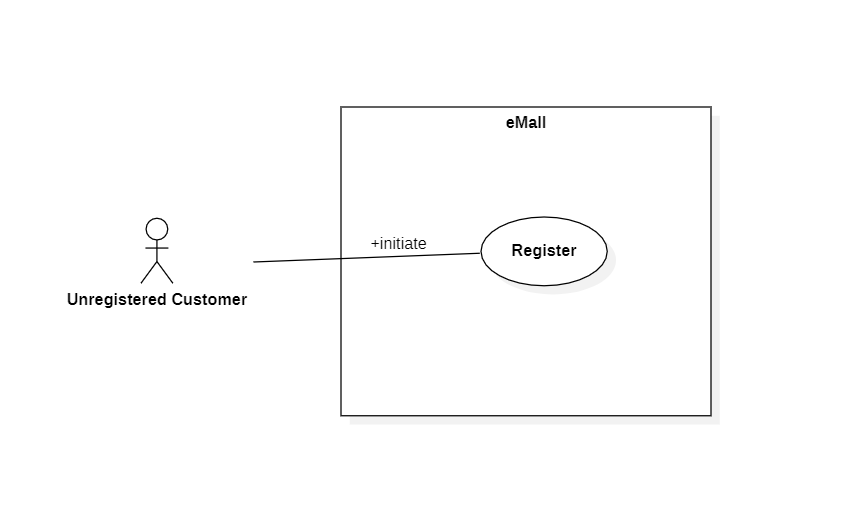
\includegraphics[width=\textwidth]{img/Unregistered_customer.PNG}
            \caption{Unregistered Customer - Use Case Diagram}
        \end{center}
    \end{figure}

    %\item \textbf{Registered Customer}
    %\begin{figure}[H]
     %   \begin{center}
      %      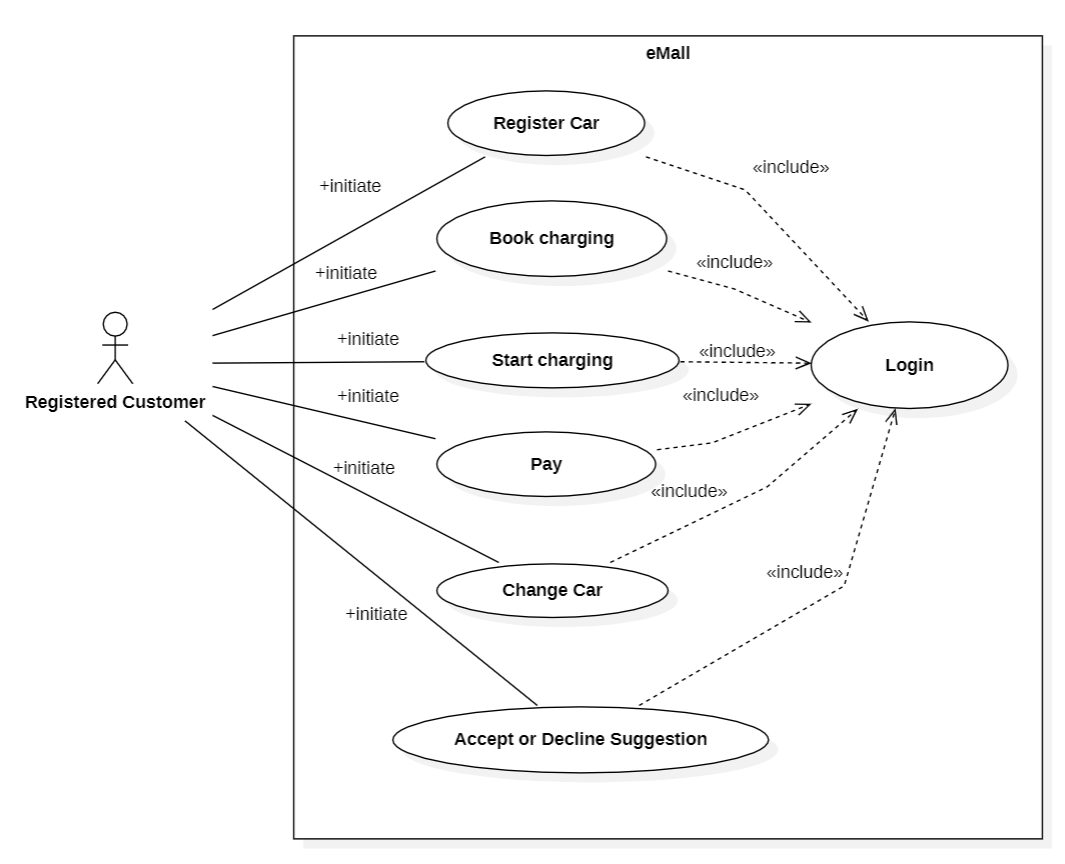
\includegraphics[width=\textwidth]{img/Registered_customer.PNG}
       %     \caption{Registered Customer - Use Case Diagram}
        %\end{center}
    %\end{figure}

    \item \textbf{Charging Point Operator}
    \begin{figure}[H]
        \begin{center}
            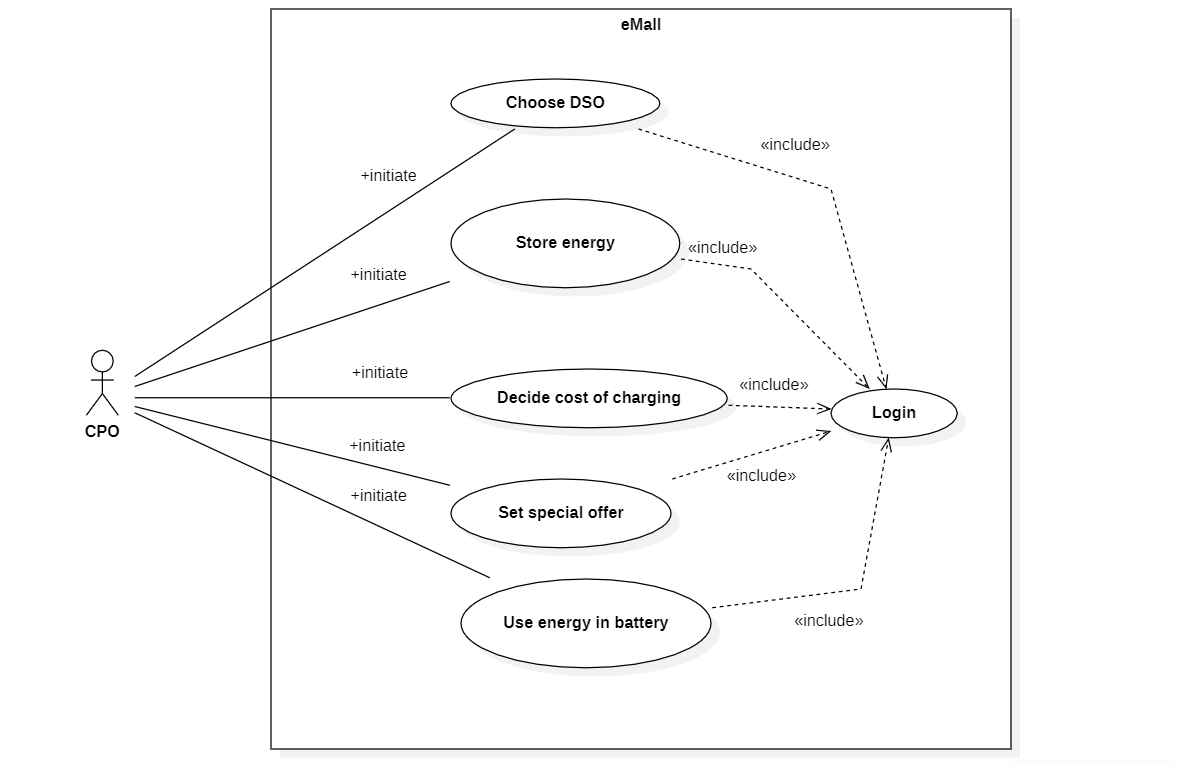
\includegraphics[width=\textwidth]{img/CPO_UseCase.PNG}
            \caption{Charging Point Operator - Use Case Diagram}
        \end{center}
    \end{figure}

\end{enumerate}
\subsubsection{Use case tables}


\subsection{Performance Requirements}
\subsection{Design Constraints}
\subsubsection{Standards Compliance}
\subsubsection{Hardware Limitations}
\subsubsection{Any Other Constraint}

\subsection{Software System Attributes}
\subsubsection{Reliability}
\subsubsection{Availability}
\subsubsection{Security}
\subsubsection{Maintainability}
\subsubsection{Portability}
